\section{Static Force Analysis} 
    A constant force (in a constant global direction) should be applied to a specific point of the output component and the force/torque needed at the driving component to keep/hold the mechanism in this position under this condition needs to be obtained from the software. This should be done with the mechanism in four positions, preferably the same four positions which were used for theoretical evaluation of kinematic parameters in Term Project 1. The point and direction of application of this force should be shown in four snapshots.

    \begin{enumerate}
        \item Position 1 
            \begin{figure}[hbt!]
                \centering
                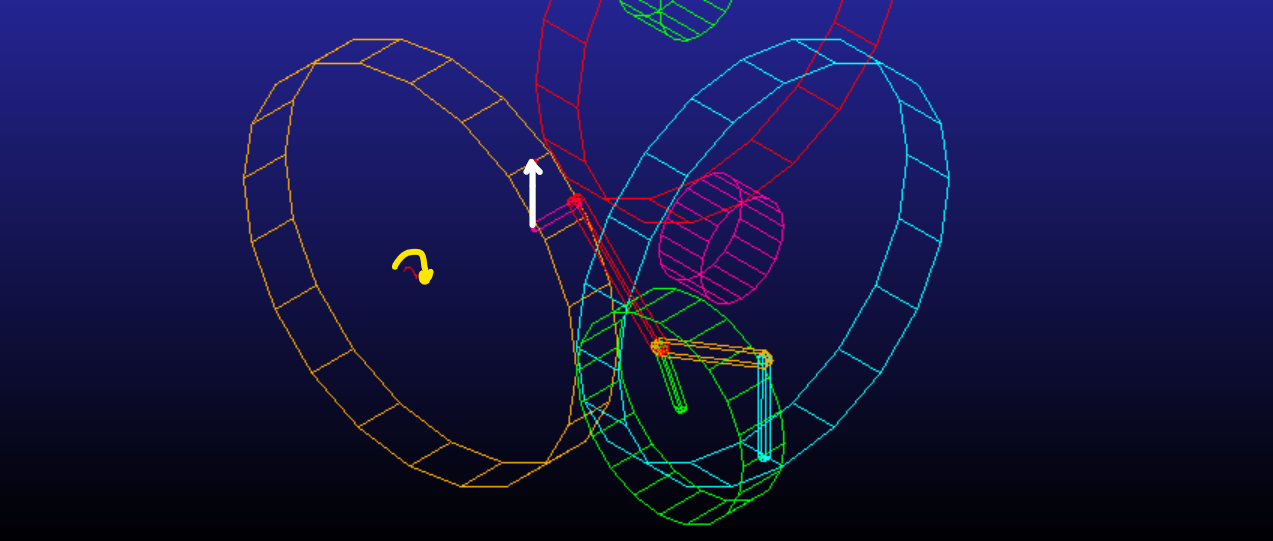
\includegraphics[width=0.9\columnwidth]{Images/Force_pos0.png}
                \caption{Mechanism and Force applied}
                \label{fig:force_applied}
            \end{figure}
            In fig~\ref{fig:force_applied}, the white arrow indicates the force applied on the output link whose magnitude is 50 kg-mm/s\^2. And the yellow curved arrow indicates the torque applied to prevent the system from moving which comes out to be -5500 kg-mm\^2/s\^2.
            \begin{figure}[hbt!]
                \centering
                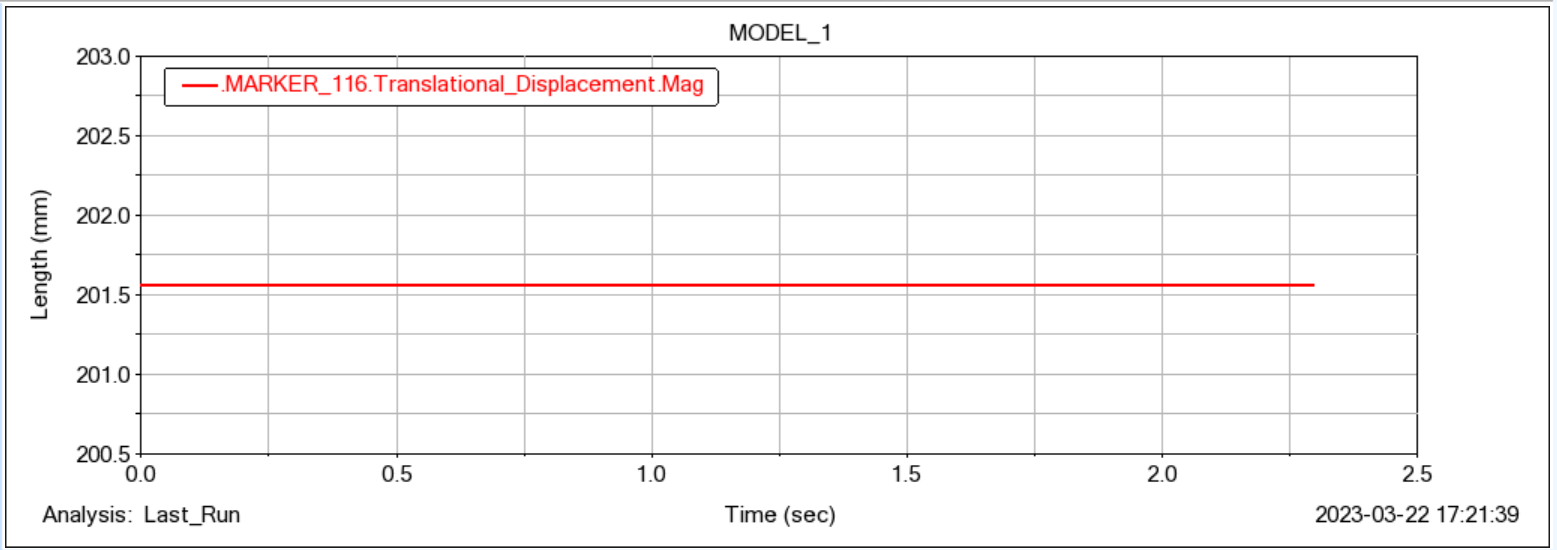
\includegraphics[width=0.9\columnwidth]{Images/Steady_output.png}
                \caption{Output displacement vs time}
                \label{fig:steady_out}
            \end{figure}
            Output displacement plot is shown in fig~\ref{fig:steady_out}, which is constant that indicates the applied torque at the input gear prevents the output link from moving.
            
            % \begin{verbatim}
            %     your
            %     code
            %     example
            % \end{verbatim}
    \end{enumerate}
            